\documentclass[11pt]{article}

\usepackage{amsmath}
\usepackage{amssymb}
\usepackage[letterpaper,margin=0.68in,headheight=15pt]{geometry}
\usepackage{array}
\usepackage{booktabs}
\usepackage{enumitem}
\usepackage{fancyhdr}
\usepackage{graphicx}
\usepackage{listings}
\usepackage{microtype}
\usepackage{tabularx}
\usepackage{tikz}
\usepackage{xcolor}
\usepackage[hidelinks]{hyperref}

\hypersetup
{
    pdftitle={ADK Lesson 017: Bounded servo intent},
    pdfauthor={Kevin Shanahan},
    pdfsubject={Bounded servo commands, Timer5 ownership, and external-power evidence},
    pdflang={en-US}
}

\usetikzlibrary{arrows.meta,positioning}
\graphicspath{{docs/lessons/assets/}{../assets/}}

\definecolor{ink}{gray}{0}
\definecolor{soft}{gray}{0.92}
\definecolor{codebg}{gray}{0.96}

\pagestyle{fancy}
\fancyhf{}
\lhead{\textsc{ADK field lesson 017}}
\rhead{Bounded servo intent}
\cfoot{\thepage}
\setlength{\parindent}{0pt}
\setlength{\parskip}{5pt}
\setlist{nosep,leftmargin=1.45em}
\renewcommand{\arraystretch}{1.18}

\lstdefinestyle{adkcpp}
{
    language=C++,
    basicstyle=\ttfamily\small,
    backgroundcolor=\color{codebg},
    frame=single,
    rulecolor=\color{ink},
    columns=fullflexible,
    keepspaces=true,
    showstringspaces=false,
    keywordstyle=\bfseries,
    breaklines=true,
    tabsize=4
}

\newcommand{\checkbox}{\(\square\)}
\newcommand{\blankline}{\rule{0.96\linewidth}{0.35pt}}
\newenvironment{checkpoint}[1]
{\begin{center}\begin{minipage}{0.94\linewidth}\textbf{Check --- #1}\par}
{\end{minipage}\end{center}}

\begin{document}

\begin{center}
    {\Huge\bfseries Separate command from motion}\\[3pt]
    {\Large Lesson 017: bounded servo intent}\\[7pt]
    \textit{Admit $\rightarrow$ command $\rightarrow$ measure
    $\rightarrow$ energize $\rightarrow$ observe}
\end{center}

\begin{center}
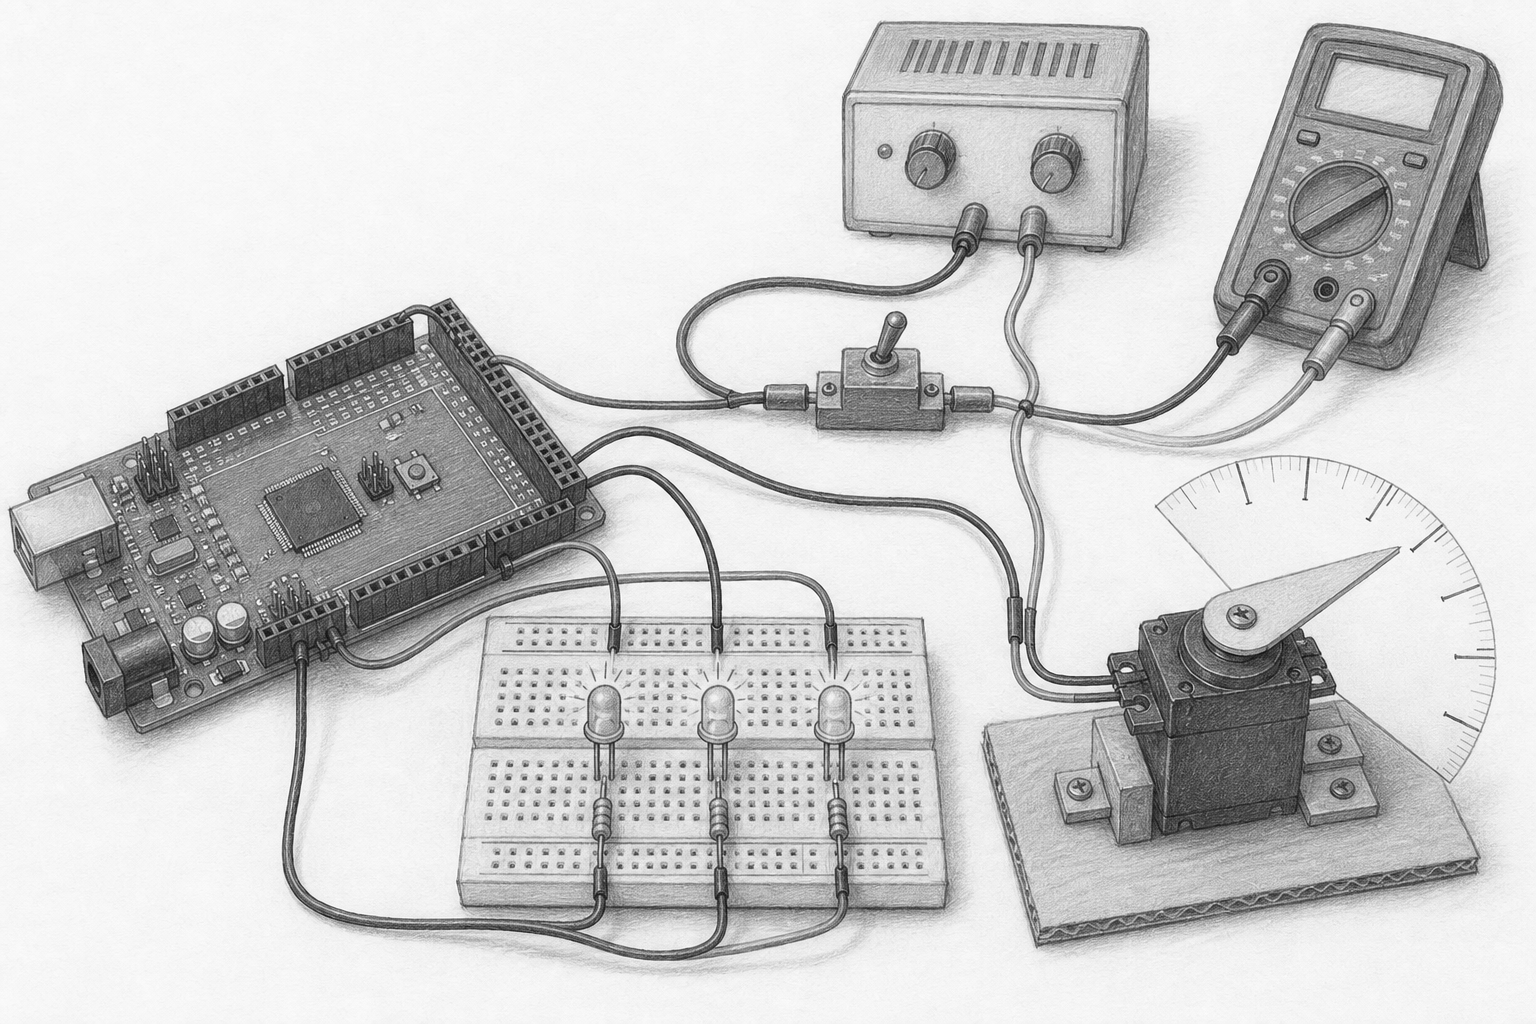
\includegraphics[width=\linewidth,height=0.31\textheight,keepaspectratio]
    {017-bounded-servo-pencil.png}
\end{center}

\textbf{Orientation plate alternative text.}
Pencil view of a Mega, three resistor-limited command-marker LEDs, a separately
powered servo carrying a paper pointer over a card, a physical supply switch,
and meter probes at the load supply. Use the schematic and table below for
exact connections.

\begin{tabularx}{\linewidth}{@{}>{\bfseries}lX@{}}
Mission & Issue one bounded command while keeping logic intent, signal,
external power, and physical position independently observable\\
Time & 120--180 minutes plus a separate reviewed bench session\\
Prerequisites & Lessons 001--016; current measurement; timer/resource ownership\\
Energy class & E2: one restrained, externally powered micro servo with no load\\
Status & Host verified and Mega compiled; physical acceptance open\\
Primary evidence & D13, D30--D32, TP-S/D44, TP-V, supply current, paper pointer\\
\end{tabularx}

\section*{1. Admit the exact physical system}

This lesson does not admit a generic ``SG90-compatible'' servo. Before
selecting a supply or pulse range, record the exact unit:

\begin{center}
\begin{tabularx}{0.96\linewidth}{@{}>{\bfseries}lX>{\bfseries}lX@{}}
Marking & & Manufacturer & \\
Primary source & & Pin order & \\
Voltage range & & Pulse range & \\
Idle/running current & & Brief start/stall limit & \\
Supply model & & Current limit & \\
\end{tabularx}
\end{center}

The first fixture carries only a soft paper pointer over a flat, taped-down
card. It has no linkage, latch, hard stop, spring, useful load, or pinch point.
The permitted software range is narrower than observed mechanical travel.
Never discover a pulse endpoint by driving into a stop.

\textbf{Stop immediately} for unexpected or reversed motion, chatter, stall,
heat, odor, current-limit operation, supply sag, reset, lost common ground,
malformed TP-S waveform, contact with the marked envelope, or disagreement
between command marker and pointer. Open the physical servo-positive switch;
do not investigate with load power present.

\section*{2. Keep the power domains explicit}

Servo positive comes from a separately regulated, current-limited supply
through a reachable physical switch or removable connector. It never connects
to Mega 5 V, VIN, USB 5 V, or an I/O pin. Join supply negative and Mega GND at
one named star point. Common ground joins signal references; it does not join
positive rails.

\begin{center}
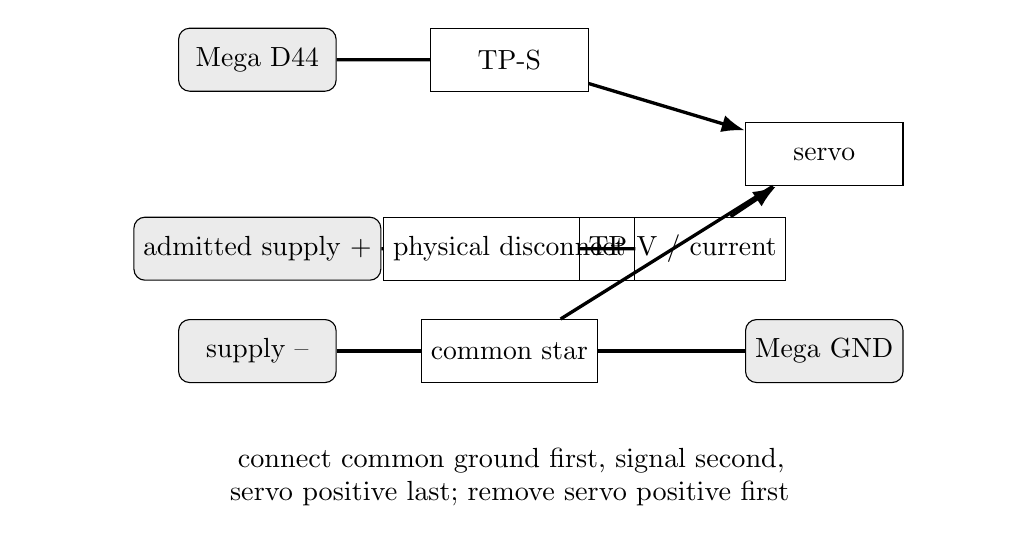
\begin{tikzpicture}[>=Latex,
    terminal/.style={draw,rounded corners,fill=soft,minimum width=20mm,
                     minimum height=8mm},
    part/.style={draw,minimum width=20mm,minimum height=8mm}]
    \node[terminal] (mega) at (0,2.4) {Mega D44};
    \node[part] (tps) at (3.2,2.4) {TP-S};
    \node[part] (servo) at (7.2,1.2) {servo};
    \draw[very thick,->] (mega)--(tps)--(servo);

    \node[terminal] (supply) at (0,0) {admitted supply +};
    \node[part] (switch) at (3.2,0) {physical disconnect};
    \node[part] (tpv) at (5.4,0) {TP-V / current};
    \draw[very thick,->] (supply)--(switch)--(tpv)--(servo);

    \node[terminal] (negative) at (0,-1.3) {supply --};
    \node[part] (star) at (3.2,-1.3) {common star};
    \node[terminal] (gnd) at (7.2,-1.3) {Mega GND};
    \draw[very thick] (negative)--(star)--(gnd);
    \draw[very thick] (star)--(servo);

    \node[below=7mm of star,text width=12cm,align=center] {
        connect common ground first, signal second, servo positive last;
        remove servo positive first};
\end{tikzpicture}
\end{center}

\begin{center}
\begin{tabularx}{\linewidth}{@{}lllX@{}}
\toprule
Evidence & Connection & Inactive state & Meaning\\
\midrule
LogicReady & D13 built-in LED & off & logic resources acquired only\\
Low/Middle/High & D30/D31/D32 through 220 \(\Omega\) LEDs & all off &
accepted command range\\
TP-S & D44/OC5C relative to Mega GND & high impedance & pulse command\\
TP-V & servo positive to supply negative & switch open & load voltage\\
Current point & series in servo-positive lead & zero with switch open &
load-domain energy\\
Pointer & soft paper on horn & unobstructed & observed shaft position\\
\bottomrule
\end{tabularx}
\end{center}

Attach meter and probe clips while all power is off. Put the current meter in
series only through the documented current point and with the correct fused
input/range. Never place a current-mode meter directly across TP-V.

\section*{3. Separate the claims}

\begin{center}
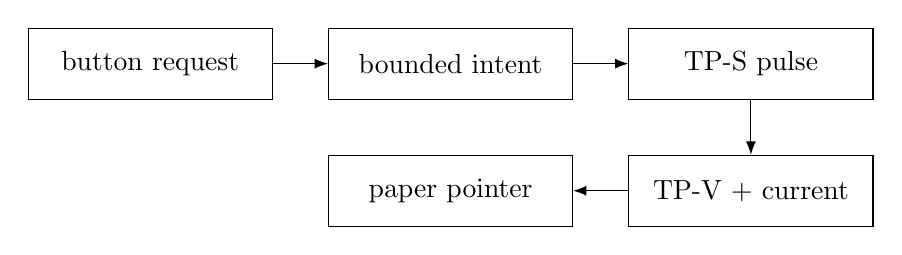
\begin{tikzpicture}[>=Latex,node distance=7mm,
    stage/.style={draw,minimum width=31mm,minimum height=9mm}]
    \node[stage] (input) {button request};
    \node[stage,right=of input] (intent) {bounded intent};
    \node[stage,right=of intent] (pulse) {TP-S pulse};
    \node[stage,below=of pulse] (power) {TP-V + current};
    \node[stage,left=of power] (pointer) {paper pointer};
    \draw[->] (input)--(intent);
    \draw[->] (intent)--(pulse);
    \draw[->] (pulse)--(power);
    \draw[->] (power)--(pointer);
\end{tikzpicture}
\end{center}

\begin{itemize}
    \item A lit marker proves the program accepted a command; it does not prove
    a pulse or motion.
    \item TP-S proves an electrical waveform; it does not prove load power.
    \item TP-V and current prove external energy; they do not prove position.
    \item The pointer shows position but supplies no controller feedback.
\end{itemize}

``Commanded middle'' and ``observed at the middle mark'' are separate record
fields. A hobby servo normally cannot report actual shaft position. Detaching
the pulse does not mechanically lock the horn. Holding a position may draw
current and is not de-energized.

\section*{4. Read the pure bounded model}

The pure model owns no pin, timer, or clock. Its position domain is 0--1000
permille; the reviewed example maps it to 1000--2000 microseconds and selects
500 as the safe position.

\begin{lstlisting}[style=adkcpp]
const adk::BoundedServoConfig servoConfig =
{
    {0, 1000, 1000, 2000},
    500
};

adk::BoundedServo servo (servoConfig);
\end{lstlisting}

\texttt{initialize()} validates the calibration and safe position but leaves
the intent \texttt{Inactive}. \texttt{command(position)} produces a
\texttt{Position} intent or rejects the position without changing the previous
accepted intent, position, or pulse. \texttt{snapshot()} returns complete
status, intent, position, and microseconds. \texttt{shutdown()} returns to
\texttt{Inactive}, \texttt{NotInitialized}, safe position, and zero pulse.

The integer interpolation is deterministic:
\[
p = p_{\min}+
 \frac{(x-x_{\min})(p_{\max}-p_{\min})}
      {(x_{\max}-x_{\min})}.
\]
The first-class record requires increasing position and pulse endpoints. The
admitted lesson record must also agree with the pointer's named direction.

\section*{5. Validate configuration without pretending storage is solved}

\texttt{ServoConfigurationRecord} has a 20-byte versioned encoding in 24 bytes
of fixed capacity. It includes calibration, safe position, generation, magic,
version, length, and CRC. It rejects erased, truncated,
future-version, checksum-failed, and semantically invalid input. It does not
silently clamp, repair, or widen a configuration.

\begin{lstlisting}[style=adkcpp]
adk::ServoConfigurationRecord record;

adk::Status status = record.save (configuration);
if (status.ok ())
{
    adk::Result<adk::ServoConfiguration> loaded = record.load ();
}
\end{lstlisting}

An empty record is \texttt{NotInitialized}; an unknown version is
\texttt{Unsupported}; corruption is \texttt{HardwareFailure}. The canonical
bench sketch encodes its reviewed compiled configuration, then decodes and
compares the complete result before acquiring any hardware resource. This
in-memory exercise defines portable bytes but does not claim EEPROM durability;
storage transport and torn-write recovery belong to the later storage lesson.

\section*{6. Own D44 and Timer5}

\texttt{MegaTimer5ServoPulseIo} is a first-class direct AVR adapter. It does
not hide Arduino's global Servo library behind the registry.

\begin{lstlisting}[style=adkcpp]
adk::ExternalPowerDomainGate powerGate;
adk::MegaTimer5ServoPulseIo  pulseIo;
adk::ServoOutput             pulseOutput (
    runtime.resources (),
    pulseIo,
    powerGate,
    adk::MegaTimer5ServoPulseIo::signalPin,
    1000,
    2000,
    adk::MegaTimer5ServoPulseIo::timer);
\end{lstlisting}

Initialization transactionally claims D44 and Timer5, then attaches an inert
endpoint. The adapter uses a 20 ms frame and writes the bounded high time to
OC5C. Timer5 ownership conflicts with PWM on D44, D45, and D46.

\texttt{ExternalPowerDomainGate::admit()} permits a command; it does not sense
or switch external voltage. That distinction lets the learner verify TP-S
while the physical servo-positive switch remains open.

Any compare-register or output-connect failure completely disables Timer5,
drives D44 low, makes D44 high impedance, and leaves the endpoint detached.
Further commands report \texttt{NotInitialized} until an explicit
shutdown/reinitialize cycle.

\section*{7. Read the canonical run loop}

The example's button advances center, low, center, and high. Its high-level
flow appears before mechanics:

\begin{lstlisting}[style=adkcpp]
const adk::TimePoint now (millis ());

if (!commandRequested (now))
{
    return;
}

const uint16_t position = positions[nextPosition];

if (!commandPosition (position))
{
    stopLogic ();
    return;
}
\end{lstlisting}

\texttt{commandPosition()} admits the command path, asks
\texttt{BoundedServo} for a pulse, sends it through \texttt{ServoOutput}, then
lights exactly one independent command marker. A fault revokes command
admission and stops the logic outputs. \texttt{stopLogic()} is intentionally
not named ``emergency stop'': the operator must still open physical servo
power.

\section*{8. Stage the first run}

\begin{enumerate}
    \item With every source off, identify the servo pins from its primary
    documentation. Mount the servo and paper pointer; mark a keep-clear arc.
    \item Connect common ground first and D44 second. Leave servo positive
    physically open. Inspect every net and probe clip.
    \item Upload and reset with servo power open. The sketch first validates
    its record, acquires D44 and Timer5, then starts the 1500 \(\mu\)s safe
    waveform and middle marker.
    \item D13 on supports completion of that startup sequence. Observe the
    TP-S high time and 20 ms frame before pressing the button and before adding
    load power.
    \item Set the exact documented voltage and current limit. Clear the arc,
    then deliberately close the physical load-power switch.
    \item Record TP-V, current, middle marker, and pointer. Press through low,
    middle, and high while remaining outside the arc.
    \item Open load power first and verify zero current. Only then stop the
    logic and verify TP-S absent and D44 high impedance.
\end{enumerate}

\begin{checkpoint}{before closing servo power}
\checkbox\ exact servo admitted \quad
\checkbox\ supply voltage/current limit recorded \quad
\checkbox\ pointer arc clear \quad
\checkbox\ D13 on \quad
\checkbox\ TP-S bounded \quad
\checkbox\ physical disconnect reachable
\end{checkpoint}

\section*{9. CLI-only workflow}

\begin{lstlisting}[style=adkcpp,language=bash]
make host-test
make arduino-Lesson017BoundedServo
make size-check
make upload EXAMPLE=Lesson017BoundedServo PORT=/dev/ttyACM0
make lessons
make lessons-check
make site
make site-check
\end{lstlisting}

Use \texttt{make boards} to find the port. Open load power before upload,
reset, or reconnect. The sketch emits no Serial data. Optional
\texttt{make monitor} and \texttt{make serial-log} records cannot replace the
marker, TP-S, TP-V, current, and pointer evidence.

The current Mega build measures 6656 bytes of flash and 323 bytes of static
RAM. Toolchain compilation is not hardware verification.

\section*{10. Diagnose from left to right}

\begin{center}
\begin{tabularx}{\linewidth}{@{}p{0.22\linewidth}p{0.36\linewidth}X@{}}
\toprule
Observation & Next check & Separation\\
\midrule
D13 off & keep load power open; inspect resource/status trace & initialization
from physical wiring\\
Marker on, no TP-S & keep load power open; inspect command admission and
Timer5 conflict & intent from pulse\\
TP-S valid, TP-V zero & inspect physical disconnect and admitted supply &
logic waveform from load power\\
TP-V sags/current limits & open power immediately; verify exact servo,
supply, polarity, and obstruction & energy source from software intent\\
Marker and TP-S agree, pointer differs & open power; inspect horn attachment,
direction, and admitted calibration & command from physical outcome\\
Chatter or heat & open power immediately; do not retry in software & unsafe
physical state from recoverable logic error\\
\bottomrule
\end{tabularx}
\end{center}

\section*{11. Deterministic proof}

Host tests enumerate calibration endpoints and overflow-safe interpolation;
invalid safe positions; record corruption at every byte; D44 and Timer5
conflicts; claim rollback; admission closed; pulse boundaries; compare and
connect failures; fail-closed teardown; repeated lifecycle calls; destruction;
and resource reuse. Injected Timer5 registers record exact ordered operations.

\begin{lstlisting}[style=adkcpp,language=bash]
make host-test
make host-test-exceptions
make quality
\end{lstlisting}

These tests prove deterministic software behavior. They cannot identify a
servo, set a supply limit, measure a pulse, or accept a physical fixture.

\section*{12. Bench acceptance record}

\begin{tabularx}{\linewidth}{@{}>{\bfseries}lX>{\bfseries}lX@{}}
Board/revision & & Sketch revision & \\
Servo identity & & Primary source & \\
Supply/current limit & & Physical disconnect & \\
Meter/probe & & Reviewer/date & \\
\end{tabularx}

\begin{center}
\begin{tabularx}{\linewidth}{@{}p{0.23\linewidth}p{0.23\linewidth}p{0.27\linewidth}X@{}}
\toprule
Claim & Prediction & Observation & Interpretation\\
\midrule
Logic acquired & D13 on; load power open & & \\
Center command & middle marker; TP-S 1500 \(\mu\)s & & \\
Low/middle/high & marker, pulse, pointer agree separately & & \\
Load power & TP-V in range; current below admitted limit & & \\
Reset/upload & load power remains physically open & & \\
Shutdown & load current zero first; TP-S absent; D44 high-Z & & \\
No back-power & asymmetric power checks meet procedure & & \\
\bottomrule
\end{tabularx}
\end{center}

\textbf{Acceptance status:}
\checkbox\ not run \quad \checkbox\ pass \quad \checkbox\ deviation attached

\section*{Exercises and next composition}

\begin{enumerate}
    \item For commands 0, 250, 500, 750, and 1000, calculate the expected
    pulse. Compare arithmetic with host snapshots before touching hardware.
    \item Corrupt each field of an exported configuration record. Predict the
    exact status and prove that no pulse intent results.
    \item Claim Timer5 or D45 PWM first. Predict the resource error and the
    unchanged TP-S state.
    \item Design a fourth evidence channel for external power without allowing
    software to switch that rail. State what it proves and what it cannot.
    \item Carry the pure bounded intent into lesson 018's inert access trainer.
    Preserve ``close requested'' separately from ``pointer observed closed.''
\end{enumerate}

Use the HTML page for maintained API links, errata, source, and copyable
commands. Use this PDF for the staged experiment, worksheets, and signed bench
record. Lesson 018 adds a keypad and display to an inert paper-pointer trainer;
it is not a lock or security product.

\section*{Primary references}

\begin{itemize}
    \item \href{https://docs.arduino.cc/hardware/mega-2560}
    {Arduino Mega 2560 Rev3 documentation and pinout}
    \item \href{https://www.microchip.com/en-us/product/atmega2560}
    {Microchip ATmega2560 Timer5 and electrical documentation}
    \item \href{https://docs.arduino.cc/libraries/servo/}
    {Arduino Servo library guidance for external power and common ground}
    \item \href{https://towerpro.com.tw/product/sg90-7/}
    {TowerPro SG90 manufacturer page---identity example, not clone authority}
\end{itemize}

\textbf{Deferred evidence.}
No physical voltage, current, waveform, travel, reset, shutdown, or
power-removal claim is accepted until a person completes this record for the
exact named fixture.

\end{document}
